\chapter{多目标隐私任务调度算法}\label{chapter:alg}

在混合云环境下,隐私任务调度问题需要同时优化完工时间、安全性以及成本三个目标,然而这些目标之间往往存在冲突。例如,提升安全性可能会延长完工时间,而降低成本可能会影响安全性。传统的优化算法使用加权求和的方式进行多目标优化,但存在着难以确定加权权重的问题。此外,而跨云协作的任务执行顺序也会影响整体调度效果。针对上述问题,本章基于多目标元启发式算法,提出了一种考虑卸载窗口优化的非支配排序遗传算法(NSGA-OW),可以同时优化兼顾完工时间、安全性与成本。

本章后续内容将详细描述算法的设计细节与实现过程。在第\ref{sec:ow-ff}节中,针对跨云协作过程中产生的虚拟机空闲时段(即卸载窗口)问题,设计了卸载窗口首次适应填充算法OW-FF。该算法通过动态检测并利用协作任务卸载至公有云时的等待时段,插入后续任务,从而提升私有云资源利用率。在第\ref{sec:nsga}节中,结合OW-FF算法提出了改进的遗传算法框架NSGA-OW,包括混合编码策略以及虚拟机分块多点交叉算子与负载感知变异算子,以加快收敛速度并提升调度质量。同时,考虑到用户对优化目标的偏好,优先优化安全性与完工时间目标,进一步提升调度速度。最后,在第\ref{sec:framework}节给出了NSGA-OW算法的流程,并分析了时间复杂度。

% NSGA-OW与OW-FF协同工作,NSGA-OW输出的虚拟机分配与安全策略决策为OW-FF提供输入,而OW-FF通过空闲时段检测进一步优化调度质量。s

\section{混合云中虚拟机资源空闲时段优化}\label{sec:ow-ff}

\begin{algorithm}[htb!]
    \caption{卸载窗口首次适应填充算法(OW-FF)}
    \label{alg:ow-ff}
    \SetAlgoLined
    \KwIn{
        $\mathcal{E}$: 任务集合,
        $\mathbf{X}$: 私有云分配矩阵,
        $\mathbf{Y}$: 公有云分配矩阵,
        $\mathbf{Z}$: 安全策略矩阵
    }
    \KwOut{任务执行序列$\mathbf{\Pi} = \{\pi_1, \pi_2, ..., \pi_S\}$}

    \For{\(i \in \{1,...,S\}\)}{
        $\mathcal{Q}_i^\text{OW} \gets \emptyset$ \tcp*[r]{初始化卸载窗口队列}
        $\pi_i \gets \emptyset$; \tcp*[r]{初始化执行队列}
    }
    \While{$\mathcal{E} \neq \emptyset $}{
        取当前任务$e_m \gets \arg\min_{e_j \in \mathcal{E}} j$\ \tcp*[r]{按任务编号升序调度}
        $\mathcal{E} \gets \mathcal{E} \setminus \{e_m\}$
        \tcp*[r]{根据私有云分配矩阵选择当前任务所在私有云虚拟机}
        $s_i$:$\exists i, \mathbf{X}[m][i]=1$;

        \If{$\mathcal{Q}_i^\text{OW} = \emptyset$}{
            \eIf{$e_m$为协作任务}{
                $w \gets \{e_w^{(\text{start})}, e_w^{(\text{end})}, \Delta\tau_w, r_w\}$\tcp*[r]{创建新的卸载窗口\(w\)}
                $e_w^\text{start} \gets e_m^{(\text{E})}$,$e_w^\text{end} \gets e_m^{(\text{V})}$\
                按式\eqref{eq:ow-span}计算$\Delta\tau_w$\  \tcp*[r]{确定卸载窗口的长度}
                $r_w \gets 5$\ \tcp*[r]{初始化失败计数器}
                $\mathcal{Q}_i^\text{OW} \gets \mathcal{Q}_i^\text{OW} \cup \{w\}$
            }{
                $\pi_i \gets \pi_i \oplus e_m^{(\text{SA})}$\ \tcp*[r]{独立任务直接加入队列}
            }
        }{
            \For{$w \in \mathcal{Q}_i^\text{OW}$}{
                \If{FT($e_m$)$\leq \text{ST}(e_w^\text{end}) \land \text{ST}(e_m) \ge \text{FT}(e_w^\text{start}) $ }{
                    $\pi_i \gets \pi_i \oplus e_w^\text{start}$\ \tcp*[r]{原开始任务加入调度队列}
                    $e_w^\text{start} \gets e_m$\ \tcp*[r]{更新开始任务}
                    \textbf{break}
                }
                \Else{
                    $r_w \gets r_w - 1$\   \tcp*[r]{插入窗口失败}
                    \tcp{删除累计5次插入失败的窗口}

                    \If{$r_w = 0$}{
                        $\mathcal{Q}_i^\text{OW} \gets \mathcal{Q}_i^\text{OW} \setminus \{w\}$
                        $\pi_i \gets \pi_i \oplus \{e_w^\text{start}, e_w^\text{end}\}$
                    }
                }
            }
        }
    }
    \Return{$\mathbf{\Pi}$}
\end{algorithm}

在混合云调度场景中,当任务以协作模式执行时,其线性工作流包含加密、公有云处理及验证三个阶段。将处理任务卸载至公有云产生的等待时延会在私有云调度中形成资源空闲时段。传统调度方法(如SPGA\cite{huangImprovedGeneticAlgorithm2023})因静态任务排序策略无法有效利用此类空闲时段(如图\ref{fig:ow-util}所示),导致跨云协作效率低下。针对该问题,本节提出卸载窗口首次适应填充算法(Offload Window FirstFit Fill,OW-FF),通过动态检测和填充协作任务执行过程中的空闲时段(即卸载窗口),优化私有云资源利用率。通过首次适应与限制测试卸载窗口次数的策略降低算法复杂度,使OW-FF在提升资源利用率的同时保持线性时间复杂度。

\begin{figure}[htb]
    % svg导入错误,不知道为什么
    % \includesvg{img/考虑和未考虑卸载窗口.drawio.svg}
    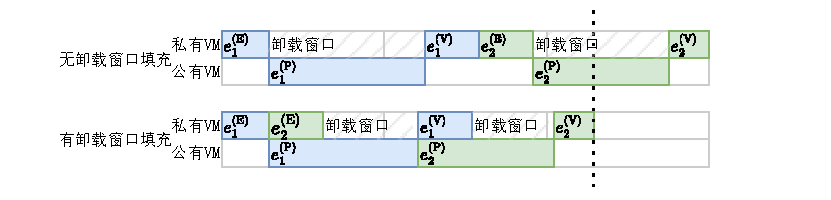
\includegraphics{img/考虑和未考虑卸载窗口.pdf}
    \caption{卸载窗口对完工时间的影响示意图}
    \label{fig:ow-util}
\end{figure}

本文将虚拟机在公私云协作过程中由于等待公有云返回处理结果而产生的资源空闲时段定义为卸载窗口(Offload Window, OW)。具体而言OW中,\( e_w^{(\text{prev})} \)表示窗口的起始任务,其完成时间\( \text{FT}(e_w^{(\text{prev})}) \)确定窗口的起始时刻;\( e_w^\text{end} \)表示窗口的终止任务,其固定为验证阶段任务\( e_m^{(\text{V})} \),其开始时间\( \text{ST}(e_w^\text{end}) \)作为窗口的终止时刻。窗口时长\( \Delta\tau_w \)限制了新任务的执行时间上限,确保插入任务不会影响后续任务的执行。当新任务插入窗口时,起始任务\( e_w^{(\text{prev})} \)更新为最后插入任务的完成时间,而终止任务\( e_w^\text{end} \)保持不变,从而维持协作任务的时序逻辑。窗口时长$\Delta\tau_w$可通过公式\eqref{eq:ow-span}计算,即:
\begin{equation}
    \Delta\tau_w = \text{ST}(e_w^\text{end}) - \text{FT}(e_w^{(\text{prev})})
    \label{eq:ow-span}
\end{equation}

OW-FF算法\ref{alg:ow-ff}通过任务集合$\mathcal{E}$与决策矩阵$\mathbf{X}$、$\mathbf{Y}$、$\mathbf{Z}$确定执行顺序$\mathbf{\Pi}$,其核心逻辑包括:任务按编号升序调度(算法第6行),确保验证任务在加密任务后执行,维持跨云协作的执行顺序依赖;当检测到协作任务时,若不存在可用卸载窗口,则以加密任务$e_m^{(\text{E})}$与验证任务$e_m^{(\text{V})}$为边界创建新窗口(算法第11-14行);通过顺序扫描窗口队列,仅允许执行时间满足$\text{FT}(e_{\text{new}})\leq\Delta\tau_w$的任务插入(算法第20行);检测到窗口可插入任务时,通过首次适应策略更新窗口起始任务并调整窗口(算法第21-22行);对于连续五次匹配失败的无效窗口,将其边界任务加入执行队列并移除窗口(算法第26-29行)。

本节提出的卸载窗口首次适应填充算法(OW-FF)通过动态检测并填充私有虚拟机因跨云协作产生的资源空闲时段,显著提升了跨云协作效率。作为NSGA-OW算法迭代循环的一部分,OW-FF采用首次适应策略与最大重试次数限制,将算法时间复杂度控制在$O(M)$,从而不会增加整体时间复杂度。同时实现近似HEFT的任务插入效果,提高了了调度质量与私有虚拟机资源利用率。

\section{遗传算法的改进}\label{sec:nsga}

本文混合云环境下隐私任务调度优化问题面临两个挑战,一是安全策略限制了虚拟机分配决策的可行位置导致搜索效率低下;二是基于遗传的元启发式算法计算速度慢。为此,本章基于NSGA-II框架提出考虑卸载窗口优化的非支配排序遗传算法(Nondominated Sorting Genetic Algorithm II with Offload Window optimization, NSGA-OW),通过混合编码策略、改进的交叉与遗传算子与动态偏好机制加快多目标优化速度,并提高调度质量。

本节介绍NSGA-OW的在遗传算法方面的改进:首先,设计了混合二进制与整数编码,解耦安全策略与虚拟机分配决策,将隐私安全约束嵌入遗传个体编解码过程,降低安全策略对搜索效率影响;其次,设计虚拟机感知与成本优化的遗传算子,在种群交叉时保留优秀的局部编码,并在变异中快速均衡负载,同时尝试关闭低负载的公有云虚拟机以降低成本;最后,设计考虑用户偏好的精英选择策略,优先优化安全性与完工时间等用户更感兴趣的指标,加快优化速度。这些改进与OW-FF算法结合,形成完整的NSGA-OW算法,为混合云环境提供了高效且安全的调度方案集合。

\subsection{混合编码方案设计}\label{subsec:nsga-encoding}

针对混合云任务调度中复杂的虚拟机分配与安全策略的决策变量,本节设计了混合编码方案,以平衡搜索效率与解的质量。私有云分配编码采用整数编码策略,每个任务\(e_m\)的私有云分配决策编码为\(X'_m \in \{1,2,\dots,S_k\}\),其中\(S_k = \sum_{i=1}^S \mathbf{L}[k][i]\)表示任务关联数据\(d_k\)在私有云中的可访问虚拟机数量。通过约束\(X'_m \leq S_k\),编码中内嵌了数据本地化约束(C2),例如当数据\(d_1\)存储在虚拟机\(s_1\)和\(s_2\)时,编码范围限定为1-2,无需额外的约束校验。公有云分配编码采用唯一索引机制,将公有云虚拟机实例映射为连续整数值\(Y'_m \in \{1,2,\dots,V_{\text{total}}\}\),其中\(V_{\text{total}} = \sum_{j=1}^J N_j\)表示公有云虚拟机总数。根据公式\eqref{eq:pubid-enumeration}将编码值转换为具体虚拟机标识符\(v_{(j,n)}\),例如当公有云提供两种类型虚拟机(类型1有3台,类型2有2台)时,编码1-5分别对应\(v_{(1,1)}, v_{(1,2)}, v_{(1,3)}, v_{(2,1)}, v_{(2,2)}\),这种线性唯一索引机制简化了公有云资源的表示。

在安全策略编码部分,针对同一隐私数据可能被多个任务共享的场景,本文提出数据安全策略编码\(Z^\text{enc}_k \in \left\{ q \mid \alpha(d_k,q) \geq \alpha_{\min}(d_k) \right\}\),其中\(k=1,2,\dots,K\)。通过为每个数据\(d_k\)独立选择满足最低安全等级的策略,而非每个任务单独决策,该机制减少了决策空间。当多个任务共享相同数据时(即\(M > K\)),决策变量减少量为\((M-K) \times Q\),同时通过限制编码范围过滤不符合最低安全要求的选项,确保约束C1的成立。任务执行模式编码采用0-1编码\(Z^{\text{offload}}_m \in \{0,1\}\),表示任务是否跨云协作,0表示私有云独立执行,1表示公有云协同处理。该编码独立于安全策略选择,允许在满足安全等级约束的前提下,根据负载动态选择执行模式以优化效率。

最终的个体编码由私有云分配、公有云分配、数据安全策略和任务协作模式四部分串联构成,表示为:
\begin{equation}
    \begin{aligned}
        \text{Individual} = &\underbrace{X'_1 \oplus \cdots \oplus X'_M}_\text{私有云分配} \oplus \underbrace{Y'_1 \oplus \cdots \oplus Y'_M}_\text{公有云分配} \\
        &\oplus \underbrace{Z^\text{enc}_1 \oplus \cdots \oplus Z^\text{enc}_K}_\text{数据安全} \oplus \underbrace{Z^{\text{offload}}_1 \oplus \cdots \oplus Z^{\text{offload}}_M}_\text{执行模式}
    \end{aligned}
\end{equation}
其中“\(\oplus\)”表示编码串联操作。通过内嵌最低安全需求约束(C1)和隐私数据存储约束(C2),该编码机制避免了约束校验与修复,同时通过压缩安全策略维度,有效降低了搜索空间复杂度,在多个任务共享同一数据的情况下可以获得更好的调度性能。

\subsection{虚拟机分块多点交叉算子}

\begin{algorithm}[htb!]
    \SetAlgoLined
    \caption{虚拟机分块多点交叉算子}\label{alg:vm-aware-cross}
    \KwIn{父代个体 $Ind_1$, $Ind_2$; 交叉概率 $p$}
    \KwOut{子代个体 $Ind_1'$, $Ind_2'$}

    初始化$\mathcal{S}_{\rm init} \leftarrow \emptyset$\;
    \ForEach{私有云虚拟机 $s \in \mathcal{S}$}{
        \If{$\text{rand}() < p$}{
            $\mathcal{S}_{\rm init} \leftarrow \mathcal{S}_{\rm init} \cup \{s\}$ \tcp*[r]{筛选待交换的私有云虚拟机}
        }
    }

    初始化$\mathcal{E}'_1 \leftarrow \emptyset,\ \mathcal{E}'_2 \leftarrow \emptyset$\;
    \ForEach{$s \in \mathcal{S}_{\rm init}$}{
        $\mathcal{E}'_1 \leftarrow \mathcal{E}'_1 \cup \{ e_m \mid Ind_1.X_m = s \}$ \tcp*[r]{收集个体1中s上的任务}
        $\mathcal{E}'_2 \leftarrow \mathcal{E}'_2 \cup \{ e_m \mid Ind_2.X_m = s \}$ \tcp*[r]{收集个体2中s上的任务}
    }

    \(Ind_1' \gets Ind_1\);
    \(Ind_2' \gets Ind_2\)\tcp*[r]{初始化子代个体}

    \ForEach{$e_m \in \mathcal{E}'_1$}{
        $Ind_2'.X_m \leftarrow Ind_1.X_m$ \tcp*[r]{交换私有云分配编码}
        $Ind_2'.Y_m \leftarrow Ind_1.Y_m$ \tcp*[r]{交换公有云实例编码}
        $Ind_2'.Z^\text{offload}_m \leftarrow Ind_1.Z^\text{offload}_m$ \tcp*[r]{交换卸载决策编码}
    }

    \Return{$Ind_1'$, $Ind_2'$}
\end{algorithm}

在混合云隐私任务调度场景中,任务分配的质量直接影响卸载时隙的利用率与虚拟机负载均衡状态,进而对完工时间等优化目标产生显著影响。传统多点交叉算子对任务编码序列进行独立交叉操作,难以保持虚拟机内部任务分配的执行顺序,容易破坏已优化的卸载窗口结构,导致调度性能下降。针对这一问题,本节提出了一种虚拟机分块多点交叉算子,其核心创新在于将交叉操作的粒度从单任务提升至虚拟机资源单元,通过以同一台私有云虚拟机作为任务分块单位进行交叉操作,从而提升NSGA-OW算法的收敛速度。

算法\ref{alg:vm-aware-cross}详细描述了虚拟机分块多点交叉算子的实现过程。在算法的3-5行中,通过交叉概率参数$p$筛选私有云虚拟机集合$\mathcal{S}_{\rm init}$作为待交换的基因,这一步骤确保了交叉操作能够以虚拟机为单位交换两个个体中的任务。随后,在算法的9-10行中,分别在父代个体中收集与选中虚拟机关联的完整任务块$\mathcal{E}'$,该任务块不仅包含初始选定任务的私有云分配信息,还涵盖了任务的公有云分配方案及安全策略,从而确保交叉后的编码能够完整保留父代个体的优化信息。在算法的14-16行中,编码交换阶段将父代的私有云分配参数$X_m$、公有云实例选择$Y_m$以及加密卸载决策$Z^{\rm offload}_m$作为一个整体与子代个体进行合并,实现了对应虚拟机中任务的完整交换,从而保留了优秀个体的卸载窗口结构与负载均衡策略。

% 由于上一小节中制定的混合编码方案内嵌了隐私与数据约束,本小节设计的交叉算子能够在无需额外修复机制的情况下,确保交叉操作不会产生不可行解的产生。然而,尽管按照虚拟机进行分块的交换策略能够有效传播优秀分配模式并加快收敛速度,但在初始阶段完全采用虚拟机整体交换的策略可能会导致种群过早失去多样性。因此,本文在算法中保留了多点交叉算子,以避免过早收敛造成的调度质量下降。此外,考虑到私有云环境中任务依赖复杂且卸载窗口的利用率对调度性能影响显著,本交叉算子主要针对私有云任务分配进行优化,而公有云任务由于结构简单没有虚拟机内部的依赖关系,采用种群初始化阶段采用的轮询法进行修复。这种设计不仅简化了算法的实现复杂度,还显著提升了交叉操作的效率与可靠性。通过这种以虚拟机为单位的交叉机制,算法能够在继承父代优质分配模式的同时,维持虚拟机内部任务执行的时序一致性,从而在全局范围内优化卸载时隙的利用率与负载均衡状态。

由于\ref{subsec:nsga-encoding}小节设计的混合编码方案内嵌的隐私与数据约束机制,本文的交叉算子能够在不引入额外修复过程的前提下,确保交叉操作始终生成可行解。通过将交叉粒度提升至虚拟机资源单元,该算子有效继承了父代个体的优质分配模式,同时维持了虚拟机内部任务执行顺序,从而优化了卸载窗口和负载均衡状态。然而,完全采用虚拟机分块的交换策略在进化初期可能导致种群多样性过早丧失,进而引发局部收敛问题。因此,本文保留了传统多点交叉算子,保证种群多样性。

\subsection{混合云负载感知变异算子}

\begin{algorithm}[htb!]
    \SetAlgoLined
    \KwIn{父代个体 $Ind$, 变异概率 $p_0=0.05$, $p_1=0.2$}
    \KwOut{子代个体 $Ind'$}

    $Ind' \leftarrow Ind$ \tcp*[r]{初始化子代个体}
    根据公式\eqref{eq:load-average}计算负载均值$\mu_L$\;
    根据公式\eqref{eq:load-std}计算负载标准差$\sigma_L$\;

    \tcp{虚拟机分配决策变异}
    \ForEach{虚拟机 $vm \in \mathcal{S} \cup \mathcal{V}$}{
        $L(vm) \leftarrow \text{根据公式\eqref{eq:vm-load}计算}$\;
        \(p \gets \) 根据公式\eqref{eq:vm-load-prob}计算变异概率\;

        \ForEach{任务 $e_m \in \mathcal{M}_{vm}$}{
            $E \leftarrow Ind'.vm$ \tcp*[r]{提取子代个体中分配给虚拟机$vm$的任务对应的编码段}

            \ForEach{编码位 $b \in E$}{
                \If{$\text{rand}() < p$}{
                    $b \leftarrow \neg b$ \tcp*[r]{执行位翻转}
                }
    } } }

    \tcp{安全决策变异}
    \ForEach{编码位 $b \in \{Z^{\rm enc}, Z^{\rm offload}\}$}{
        \If{$\text{rand}() < p_0$}{
            $b \leftarrow \neg b$ \tcp*[r]{执行位翻转}
    } }

    \Return $Ind'$\;
    \caption{混合云负载感知变异算子}
    \label{alg:load-aware-mutation}
\end{algorithm}

对混合云调度问题的分析发现,虚拟机负载过高会使完工时间变长,而公有云虚拟机负载过低导致的资源利用率低下则造成成本目标上升。为了解决负载不均衡对完工时间与成本的负面影响,本文设计了一种负载感知的变异算子。该算子根据虚拟机负载调整变异概率提升了算法的收敛速度,并降低完工时间且优化了成本。该变异算子,针对负载过大的虚拟机,系统增加其变异概率,促使任务向负载接近均值的虚拟机迁移,从而均衡整体负载分布;对于负载过低的虚拟机,通过提高变异概率来尝试关闭负载过低的公有云虚拟机,进而降低运营成本。负载感知变异算子的具体实现详见算法\ref{alg:load-aware-mutation}。

为了准确评估混合云环境中的虚拟机负载状况,本节建立了负载计算模型,并定义了相关的统计指标。如公式\eqref{eq:vm-load}所示,虚拟机负载率可表示为:
\begin{equation} L(vm) =
    \begin{cases} \frac{\sum_{e_m \in \mathcal{M}_i} o_{\text{proc}}\times \text{size}(e_m)}{A_i}, & vm \in \mathcal{S}\quad \text{(私有云虚拟机)} \\ \frac{\sum_{e_m \in \mathcal{M}_i} o_{\text{proc}}\times \text{size}(e_m)}{B_j}, & vm \in \mathcal{V}\quad \text{(公有云虚拟机)}
    \end{cases} \label{eq:vm-load}
\end{equation}
其中,$\mathcal{M}_i$表示分配到虚拟机$vm$的任务集合,$A_i$为私有云虚拟机$s_i$的计算能力(单位:MHz),$B_j$为公有云虚拟机类型$j$的计算能力(单位:MHz),$o_{\textup{proc}}$表示任务$e_m$的计算量(单位:CPU周期)。

在排除没有任务的虚拟机后,本文对虚拟机的负载情况进行统计分析,分别计算其负载均值与标准差,如公式\eqref{eq:load-average}和\eqref{eq:load-std}所示。
负载均值$\mu_L$表示所有活跃虚拟机负载的平均值,计算公式为:
\begin{equation}
    \mu_L = \frac{1}{N} \left( \sum_{s_i \in \mathcal{S}} L(s_i) + \sum_{v_{(j,n)} \in \mathcal{V}} L(v_{(j,n)}) \right)
    \label{eq:load-average}
\end{equation}

负载标准差$\sigma_L$则用于衡量虚拟机负载与平均值的平均距离,计算公式为:
\begin{equation}
    \sigma_L^2 =  \frac{1}{N} \left(
        \sum_{s_i \in \mathcal{S}} (L(s_i) - \mu_L)^2 + \sum_{v_{(j,n)} \in \mathcal{V}} (L(v_{(j,n)}) - \mu_L)^2
    \right)
    \label{eq:load-std}
\end{equation}
其中$N$为活跃虚拟机总数。基于上述统计指标,本文设计了根据虚拟机负载调整变异概率公式:
\begin{equation}
    p =
    \begin{cases}
        p_0 + \dfrac{|L_v - \mu_L|}{3\sigma_L} \cdot (p_1 - p_0), & |L_v - \mu_L| \leq 3\sigma_L \\
        p_1, & |L_v - \mu_L| > 3\sigma_L
    \end{cases}
    \label{eq:vm-load-prob}
\end{equation}
该公式通过变异最低概率$p_0$与最大概率$p_1$,调整变异算子的位翻转变异概率。对于负载偏离平均值的虚拟机,其变异概率会相应增加,从而促进混合云负载均衡,并尝试关闭关闭负载过低的公有云节点。

\subsection{考虑用户偏好的精英保留策略}

NSGA-II算法作为一种基于遗传算法的多目标优化方法,虽然具备全局搜索能力强、调度质量高以及提供多样化调度方案的优点,但其收敛速度较慢。在混合云隐私任务调度场景中,完工时间的优化直接影响用户体验,而安全性的提升可以降低隐私数据潜在风险。相比之下,成本目标由于公有云资源的规模效应,其对调度质量的影响相对较小。因此,本文设计了考虑用户偏好的精英保留策略,优先优化安全性与完工时间,以加快调度速度。该策略保留了原始精英选择机制的核心,即通过非支配排序保留精英解以加速收敛,同时利用拥挤度排序维持种群多样性。与原始策略不同,本文通过动态生成权重对拥挤度函数进行加权,引导算法优先优化用户关注的关键目标。同时,参考随机分配权重策略的研究\cite{wangIntegratingWeightAssignment2018},每轮迭代中动态调整权重,既引导算法优先优化关键目标,又通过多样化的搜索方向避免静态加权导致的过早收敛问题,从而降低丢失全局最优解的风险。

\begin{algorithm}[htb!]
    \SetAlgoLined
    \caption{考虑用户偏好的精英保留策略}\label{alg:pref-elite-choose}
    \KwIn{非支配排序后的当前种群 \(P = \{F_1, F_2, \dotsc, F_k\}\);子代规模 \(N\)}
    \KwOut{子代种群 \(P'\)}
    \(P' \gets \emptyset\) \tcp*{初始化子代种群}
    \(i \gets 1\)

    \While{ \( |P'| + |F_i| \leq N \) } {
        \(P' \gets P' \cup F_i\) \tcp*{保留精英个体}
        \(i \gets i+1\)
    }

    \Repeat{满足 \(w_1 > w_2 \land w_3 > w_2 \)}{
        随机生成偏好权重\(w_1, w_2, w_3 \sim \text{rand}()\)
    }
    根据公式\eqref{eq:crowd-with-pref}改进的拥挤度\(\text{Crowd}'(s)\)降序排列\(F_i\) \\
    选取前\(N - |P'|\)个个体加入\(P'\)
    \While{\(|P'| < N\)}{
        \(P' \gets P' \cup \{F_i[1]\}\) \tcp*{选择拥挤度最高的非精英个体}
        \(F_i \gets F_i[1:]\)
    }
    \Return \(P'\)
\end{algorithm}

具体来说,算法在每次拥挤度计算时随机生成三个权重,并约束安全性与完工时间的权重大于成本目标,确保优化资源向关键目标集中。这允许个体在这两个方向上分布更为密集,以便实现更深入的优化;而在优化成本的方向,减少个体分布密度,从而将更多资源用于优化用户更关注的目标。本文将动态权重在拥挤度计算中考虑用户偏好,从而使优化算法优先优化关键目标。改进的拥挤度计算如公式\eqref{eq:crowd-with-pref}所示:
\begin{equation}
    \text{Crowd}'(s) = w_1 \cdot (1-\text{norm}(\text{Makespan})) + w_2 \cdot \text{norm}(\text{Security}) + w_3 \cdot (1-\text{norm}(\text{Cost}))
    \label{eq:crowd-with-pref}
\end{equation}
其中\(\text{norm}(\cdot)\)表示目标值的归一化处理函数。对于需要最小化的完工时间与成本目标,采用\(1-\text{norm}(\cdot)\)的形式进行处理,使得目标值越小拥挤度越大;对于需要最大化的安全性目标,直接使用\(\text{norm}(\cdot)\)进行转换,确保安全性越高拥挤度越大。算法的具体流程如算法\ref{alg:pref-elite-choose}所示,其核心在于动态调整权重以引导优化方向。每次执行精英选择时,随机生成权重\(w_1, w_2, w_3 \in [0,1]\),并满足约束条件\(w_1 > w_2\)且\(w_3 > w_2\),以确保完工时间与安全性的权重始终高于成本目标。

% \subsection{考虑卸载窗口优化的非支配排序遗传算法流程}

% 本节详细描述NSGA-OW算法的完整执行流程,其核心逻辑如图\ref{fig:mhalg-flow}所示。算法通过分层迭代机制实现混合云隐私任务的多目标调度优化,具体步骤如下:
% 在本章,我们在\ref{sec:ow-ff}节设计了优化混合云资源空闲时段的OW-FF算法,在本节改进了NSGA-II的交叉、变异遗传算子与精英选择策略,现在我们可以使用这些算法,完成NSGA-OW算法框架。本文提出的NSGA-OW整体的优化流程如图\ref{fig:mhalg-flow}所示,通过卸载窗口首次适应(OW-FF)算法优化空闲资源时段并使用针对问题改进的NSGA-II算法最终求解第\ref{chapter:model}章提出的多目标优化问题。

\section{考虑卸载窗口优化的非支配排序遗传算法}\label{sec:framework}

% 在本章的前面章节中,我们已逐步实现了NSGA-OW算法框架的核心组件:首先,针对混合云资源空闲时段的优化问题,设计了卸载窗口首次适应填充算法(OW-FF),通过动态检测与填充私有虚拟机因跨云协作产生的空闲时段,显著提升了资源利用率;其次,基于NSGA-II框架,提出了虚拟机分块多点交叉算子与负载感知变异算子,通过优化遗传操作提升算法的收敛效率;最后,引入考虑用户偏好的精英选择策略,优先优化安全性与完工时间目标,同时兼顾成本控制。在此基础上,本节将上述组件整合为完整的NSGA-OW算法框架,通过协同优化机制实现混合云隐私任务的多目标调度优化。如图\ref{fig:mhalg-flow}所示,NSGA-OW通过结合了OW-FF检测空闲时间与多目标遗传算法进行虚拟机与安全策略决策,一方面,虚拟机分配与安全策略决策为OW-FF提供输入参数,优化任务执行顺序;另一方面,OW-FF生成的任务时序反馈至目标函数,为遗传算法提供精确的调度质量评估。这种协同设计提升了调度质量。

在本章的前面章节中,我们已逐步实现了NSGA-OW算法框架的各个组件:首先,设计了卸载窗口首次适应填充算法(OW-FF),用于动态检测与填充私有虚拟机因跨云协作产生的空闲时段;其次,设计了虚拟机分块多点交叉算子与负载感知变异算子,交叉算子可以交换个体的编码提升收敛速度,变异算子可以为种群引入新编码提升全局搜索性能;最后,引入考虑用户偏好的精英选择策略,在非支配排序过程中优先优化安全性与完工时间目标以加快算法执行速度。在此基础上,本节将上述组件整合为完整的NSGA-OW算法框架,通过协同优化机制实现混合云隐私任务的多目标调度优化。NSGA-OW算法流程如图\ref{fig:mhalg-flow}所示。

\subsection{算法流程}

\textbf{种群初始化:}
为了产生良好的初始种群,本文采用随机初始化策略生成规模为$N$的初始种群。对于每个个体,依据公式\eqref{eq:random-init}随机生成遗传编码,具体包括虚拟机分配$X'_m$、公有云映射$Y'_m$、数据加密策略$Z^\text{enc}_d$及安全方法选择$Z^\text{method}_m$。其中,虚拟机分配$X'_m$在可用虚拟机范围内随机选择,公有云映射$Y'_m$在公有云的虚拟机范围内内生成,数据加密策略$Z^\text{enc}_d$从满足最低安全需求的策略集合中随机选取,而安全方法选择$Z^\text{method}_m$是随机的0-1编码。该初始化策略确保了种群的多样性,为后续遗传操作提供了充分的搜索空间。

\textbf{空闲时段检测与目标函数计算:}
对当前种群中的每个个体,调用算法\ref{alg:ow-ff}进行空闲时段检测与任务排序,根据遗传编码确定的私有虚拟机分配矩阵$\mathbf{X}$、公有云分配矩阵$\mathbf{Y}$及安全策略$\mathbf{Z}$,该阶段利用首次适应规则检测并尝试将任务插入空闲时段,同时通过重试限制策略将算法复杂度控制在\(O(M)\)。完成调度编排后,分别计算个体的三个目标函数值:完工时间\(\text{Makespan}\)、安全性\(\text{Security}\)及成本\(\text{Cost}\)。

\begin{equation}
    \begin{aligned}
        % 随机生成
        X'_m &= \text{round}\left(\text{rand}(0,1) \cdot \sum_{i \in S}\mathbf{L}[d][i]\right)  \\
        Y'_m &= \text{round}\left(\text{rand}(0,1) \cdot \sum_{j \in J}N_j\right)  \\
        Z^\text{enc}_d &= \text{round}\left(\text{rand}(0,1) \cdot \sum_{k \in K}\mathbb{I}(\alpha(d_k,q) \geq \alpha_{\min}(d_k))\right)  \\
        Z^\text{method}_d &= \text{round}\left(\text{rand}(0,1)\right) \\
        \label{eq:random-init}
    \end{aligned}
\end{equation}
其中,\(\sum_{i \in S}\mathbf{L}[d][i]\)表示存储任务隐私数据的可用虚拟机数,\(\sum_{j \in J}N_j\)为公有云虚拟机总数,\(\sum_{k \in K}\mathbb{I}(\alpha(d_k,q) \geq \alpha_{\min}(d_k))\)统计符合最低安全需求的策略数。

% \textbf{非支配排序与考虑用户偏好的精英选择}
% 将父代与子代种群合并后,采用快速非支配排序算法分层,形成前沿层级集合$\{F_1, F_2,...,F_k\}$。执行算法\ref{alg:pref-elite-choose}进行精英保留:首先将完整加入的前沿层级填充至下一代种群,若剩余名额存在于临界前沿$F_i$,则依据改进拥挤度$\text{Crowd}'(s)$(公式\eqref{eq:crowd-with-pref})选取个体,其中动态权重$w_1$、$w_2$、$w_3$确保安全性与完工时间的优化优先性。

\textbf{交叉与变异遗传操作生成新种群:}
对经过非支配排序与精英选择后的个体执行遗传进化操作。在交叉操作中,采用混合普通多点交叉与虚拟机分块多点交叉(算法\ref{alg:vm-aware-cross})的策略,其中后者以概率$p$选取私有云虚拟机作为交换单元,整体迁移其关联任务的分配方案,保留优质调度模式的同时加速种群收敛。在变异操作中,执行负载感知变异(算法\ref{alg:load-aware-mutation}),根据虚拟机负载偏离均值的程度调整位翻转概率(公式\eqref{eq:vm-load-prob}),从而使虚拟机间负载均衡,并提升种群的多样性。这种混合遗传操作的设计不仅继承了传统NSGA-II算法的探索能力,还通过虚拟机分块与负载感知机制强化了局部搜索效率,有效提升了调度质量与算法的收敛速度。

\textbf{非支配排序与考虑用户偏好的精英选择:}
将交叉与变异操作产生子代种群与负载种群合并后,采用快速非支配排序算法分层,形成前沿层级集合$\{F_1, F_2,...,F_k\}$。随后,应用考虑用户偏好的精英选择策略(算法\ref{alg:pref-elite-choose})进行筛选优秀个体进入下一轮迭代。改进的精英选择策略不仅保留了传统NSGA-II算法的多样性维持能力,还通过偏好引导机制提升了关键目标方向的搜索效率,从而加快调度算法速度。

\textbf{迭代终止判断:}
重复执行空闲时段检测至用户偏好的精英保留步骤,直至达到预设迭代次数$T$。最终输出包含非支配解集的Pareto前沿解集,各解在安全、时效与成本分布均匀,用户可根据实际需求选择最优调度方案。

\begin{figure}
    % \includesvg[width=0.8\textwidth]{img/nsgaow.svg}
    % \includesvg{img/nsgaow流程图.drawio.svg}
    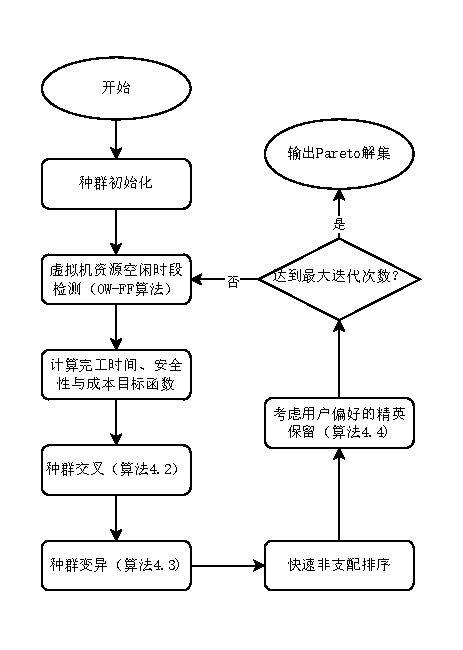
\includegraphics{img/nsgaow流程图.drawio.pdf}
    \caption{NSGA-OW算法流程示意图}\label{fig:mhalg-flow}
\end{figure}

\subsection{时间复杂度分析}

接下来分析NSGA-OW的时间复杂度。原始NSGA-II算法的时间复杂度主要取决于种群规模\(L\)、迭代次数\(T\)、交叉变异算子以及非支配排序的计算开销。在NSGA-OW框架中,单个个体的编码由任务分配、虚拟机选择和安全策略三部分构成,编码总长度为\(3M + K\),其中\(M\)表示任务总数,\(K\)表示隐私数据数量,且满足\(K \le M\),\(S\)表示私有虚拟机数量。

首先,分析NSGA-OW对每个个体的处理开销。原始的多点交叉与位翻转变异算子的时间复杂度为线性,由于隐私数据数量\(K\)少于等于任务数量\(M\),其时间复杂度为 \(O(M)\)。虚拟机分块多点交叉算子在基础交叉操作上增加了私有云虚拟机的筛选与关联任务块的查找操作,其时间复杂度分别为 \(O(S)\) 和 \(O(M)\),通常情况下任务的数量\(M\)多于私有云虚拟机的数量\(S\),因此整体复杂度仍为 \(O(M)\)。混合云负载感知变异算子增加了计算虚拟机负载均值与标准差步骤,其时间复杂度保持不变,为 \(O(M)\)。此外,关于卸载窗口首次适应填充算法(OW-FF)的时间复杂度,考虑最复杂的优化场景,即每个任务均在协作处理模式下运行。定义任务的分配与比较为一次单位操作。在此场景下,每个任务包含3个子任务,算法按任务下标顺序分配任务,其中公有云任务仅需进行一次分配操作。私有云中维护的卸载窗口队列,在每次窗口匹配失败的最差情况下,每个任务需要分配一个卸载窗口,且每个窗口由于最大重试次数限制最多比较5次。综上所述,每个任务最多产生7次单位操作,作为常数项时间复杂度可以忽略。因此,OW-FF算法的时间复杂度为 \( O(M) \)。因此,NSGA-OW对每个个体的处理时间复杂度为 \(O(M)\)。最后,本文为三目标优化算法,快速非支配排序需要每个个体与其他个体进行比较,其时间复杂度为 \(O(L^2)\),。因此,NSGA-OW每次迭代的时间复杂度为 \(O(L^2)\)。

综上所述,NSGA-OW的总时间复杂度为 \(O(TL^2 + TLM)\),其时间复杂度与迭代次数\(T\),种群数量\(L\)以及任务数量\(M\)有关,与原始NSGA-II保持一致。上述分析表明,本文设计的变异、交叉算子以及OW-FF算法并未增加原算法的时间复杂度,在保证优化性能的同时,维持了NSGA-II快速非支配排序算法在时间复杂度上的优势。

\section{本章小结}

本章针对混合云环境下隐私任务多目标调度优化问题展开研究,提出了一种考虑卸载窗口优化的非支配排序遗传算法NSGA-OW。首先,针对跨云协作过程中虚拟机空闲时段导致资源利用率低下的问题,设计了卸载窗口首次适应填充算法(OW-FF)。该算法通过动态检测空闲时段并引入重试限制策略,将时间复杂度控制在\( O(M) \)内,可以与遗传算法框架整合。其次,根据多目标优化问题的特点,设计混合编码方案,并通过内嵌约束规则减少不可行解的出现次数,从而提高搜索效率。在此基础上,设计了遗传算子组合:虚拟机分块多点交叉算子以虚拟机为单位交换任务分配方案,确保优质分配模式的完整继承;负载动态变异算子则根据虚拟机负载动态调整变异概率,优化完工时间与运营成本。最后,设计带偏好的精英选择策略,通过随机加权方式引导算法优先优化安全性与完工时间目标,加快关键目标的搜索速度。算法性能方面,改进的NSGA-OW的时间复杂度与NSGA-II算法相同,保持了NSGA-II算法的高效性。

